\section{Selected Distributions for Statistics}\label{app:dist}
%%%%%%%%%%%%%%%%%%%%%%%%%%%%%%%%
%%
\renewcommand{\theexmp}{\Alph{section}.\roman{exmp}}
%%%%%%%%%%%%%
\begin{exmp}[Normal distribution]{exmp:normald}
	The Normal distribution, also known as Gaussian, is the most common distribution form and can often be observed in nature. The bell-shape is characteristic. It is characterized by the mean $\mu$ and the variance $\sigma^2>0$: $\sim N(\mu,\sigma^2)$. The case of $\mu=0$ and $\sigma^2=1$ is named the Standard Normal distribution $\sim N(0,1)$.		
	
	\centering{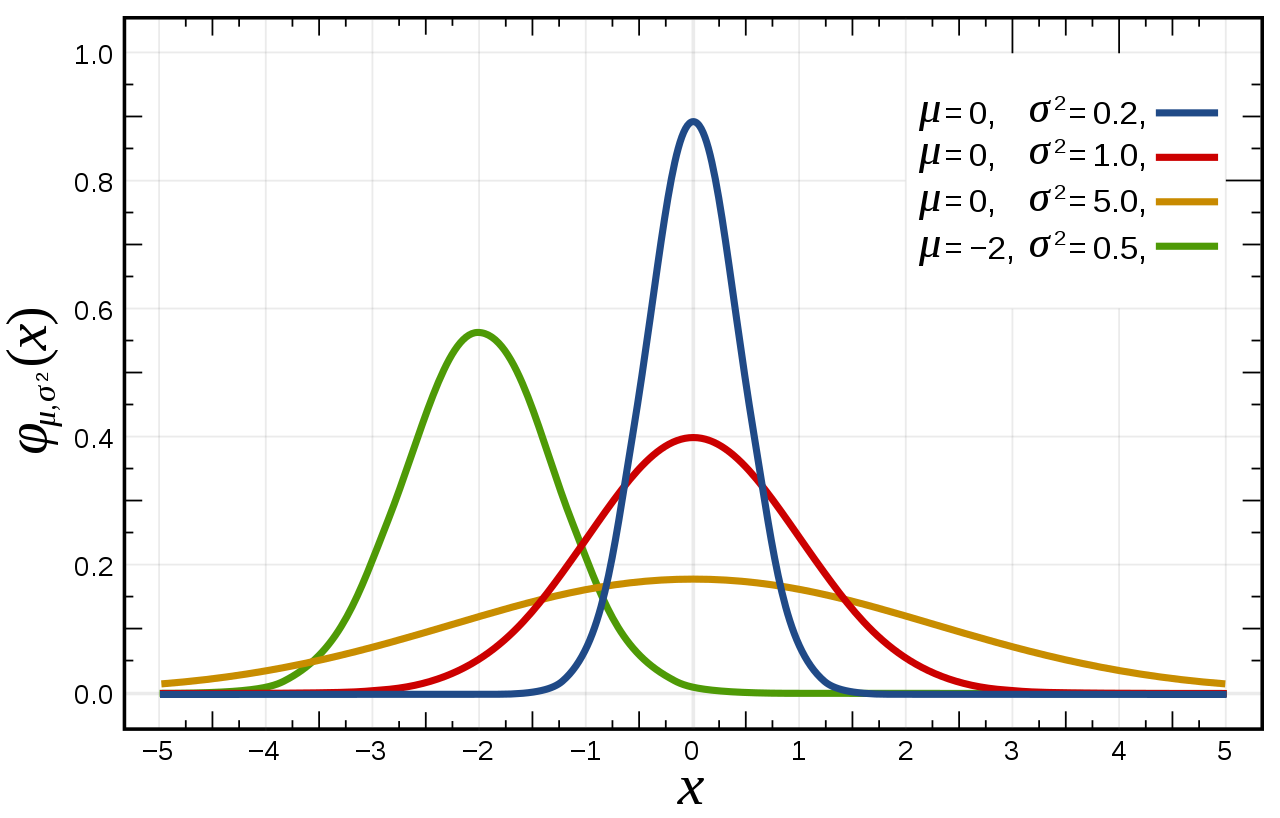
\includegraphics[height=0.36\textheight]{P01npdf.png}
	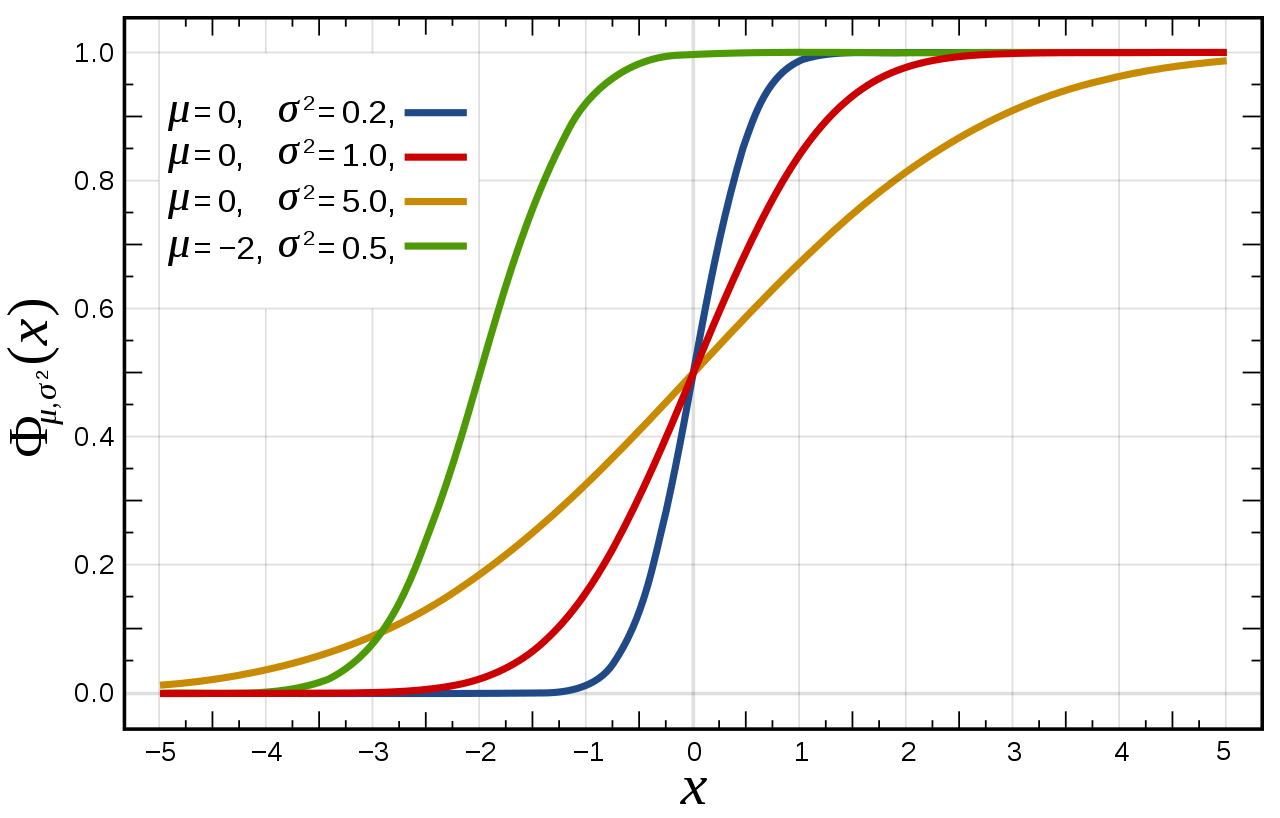
\includegraphics[height=0.36\textheight]{P02ncdf.png}}
	\credits{Public Domain.}	
\end{exmp}
\pagebreak
%%%%%%%%%%%%%%%%%%%%%%%%%%%%%%%%
\begin{exmp}[Student's t-distribution]{exmp:studentt}
	The t-distribution shows the distribution of means from a sample $n$ drawn from a normal distributed population. It is characterized by the degrees of freedom $dof=n-1$: $\sim t(dof)$.
		
	\centering{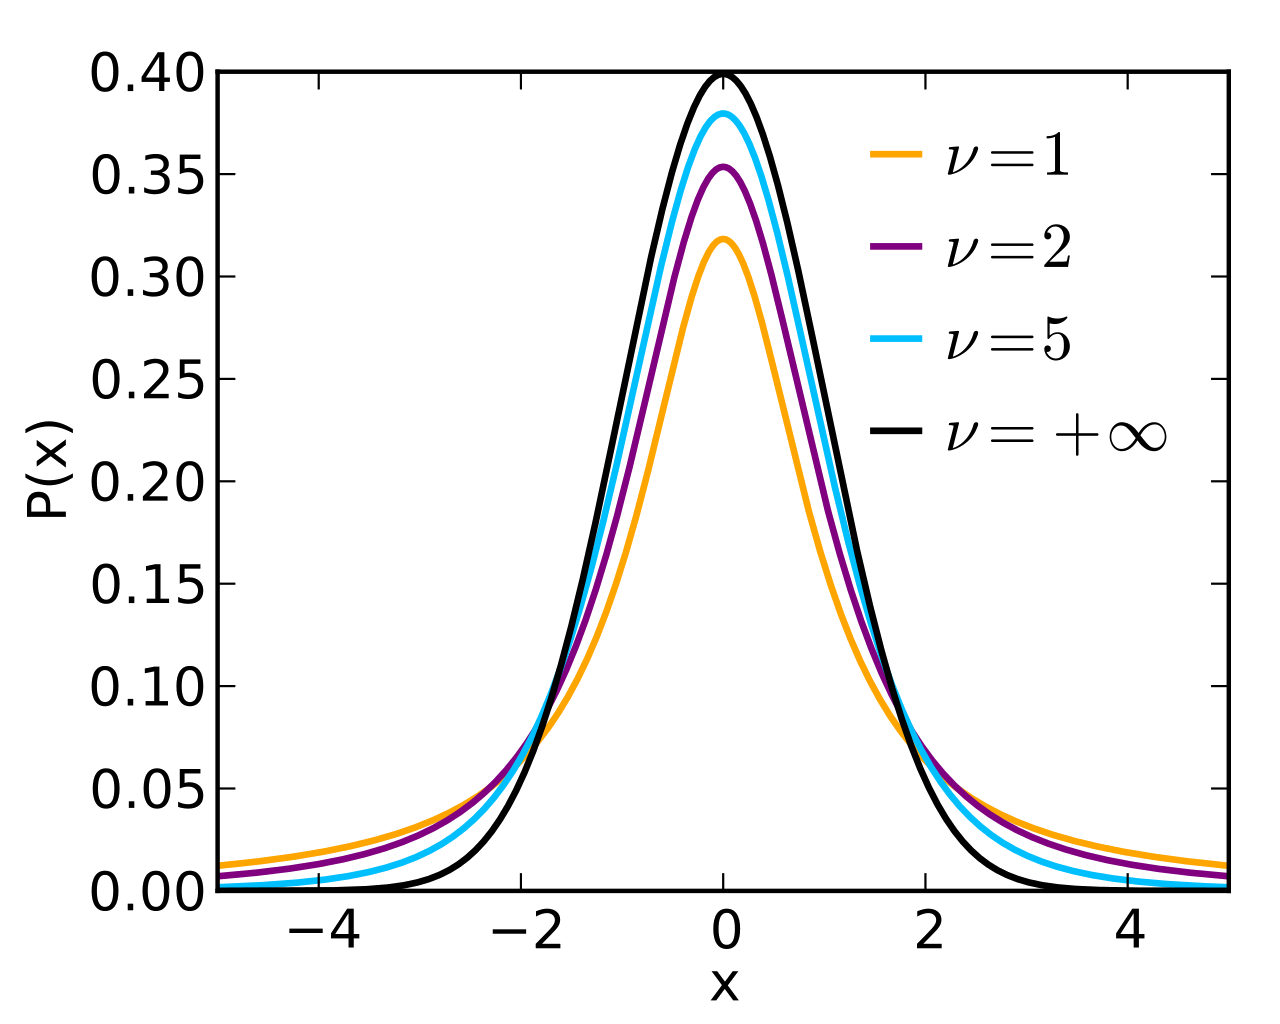
\includegraphics[height=0.38\textheight]{P03tpdf.png}
	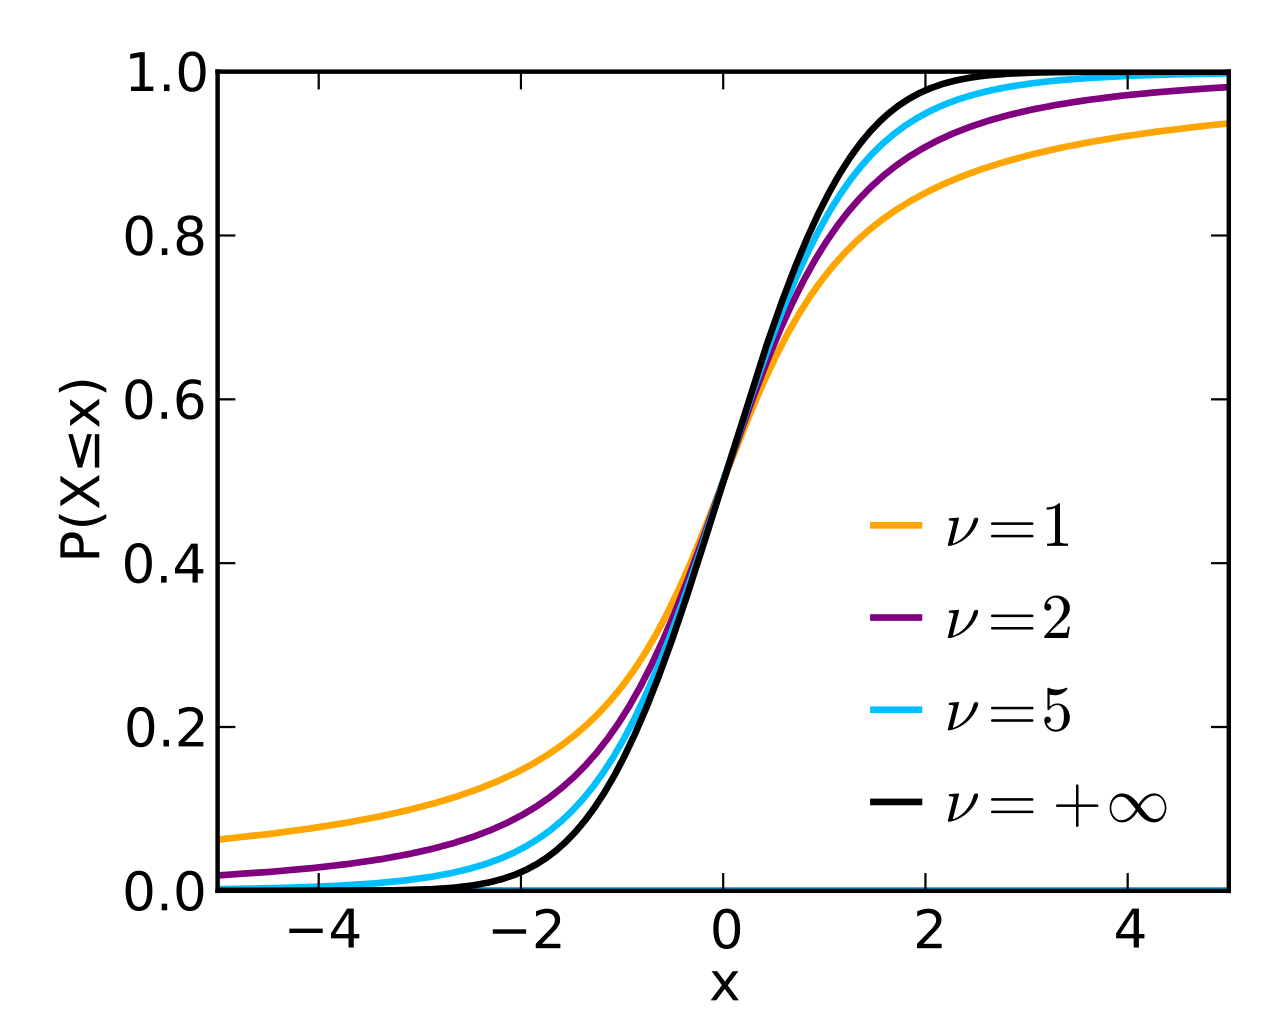
\includegraphics[height=0.38\textheight]{P04tcdf.png}}		
	\credits{By Skbkekas at Wikipedia Commons. CC BY 3.0.}
\end{exmp}
\pagebreak
%%%%%%%%%%%%%%%%%%%%%%%%%%%%%%%%
\begin{exmp}[Chi-squared distribution]{exmp:chisq}
	The $\chi^2$-distribution is the distribution of sums from $k$ independent standard normal distributions. $k$ is also named degrees of freedom and characterizing the $\chi^2$-distribution $k=dof$: $\sim \chi^2(k)$.
	
	\centering{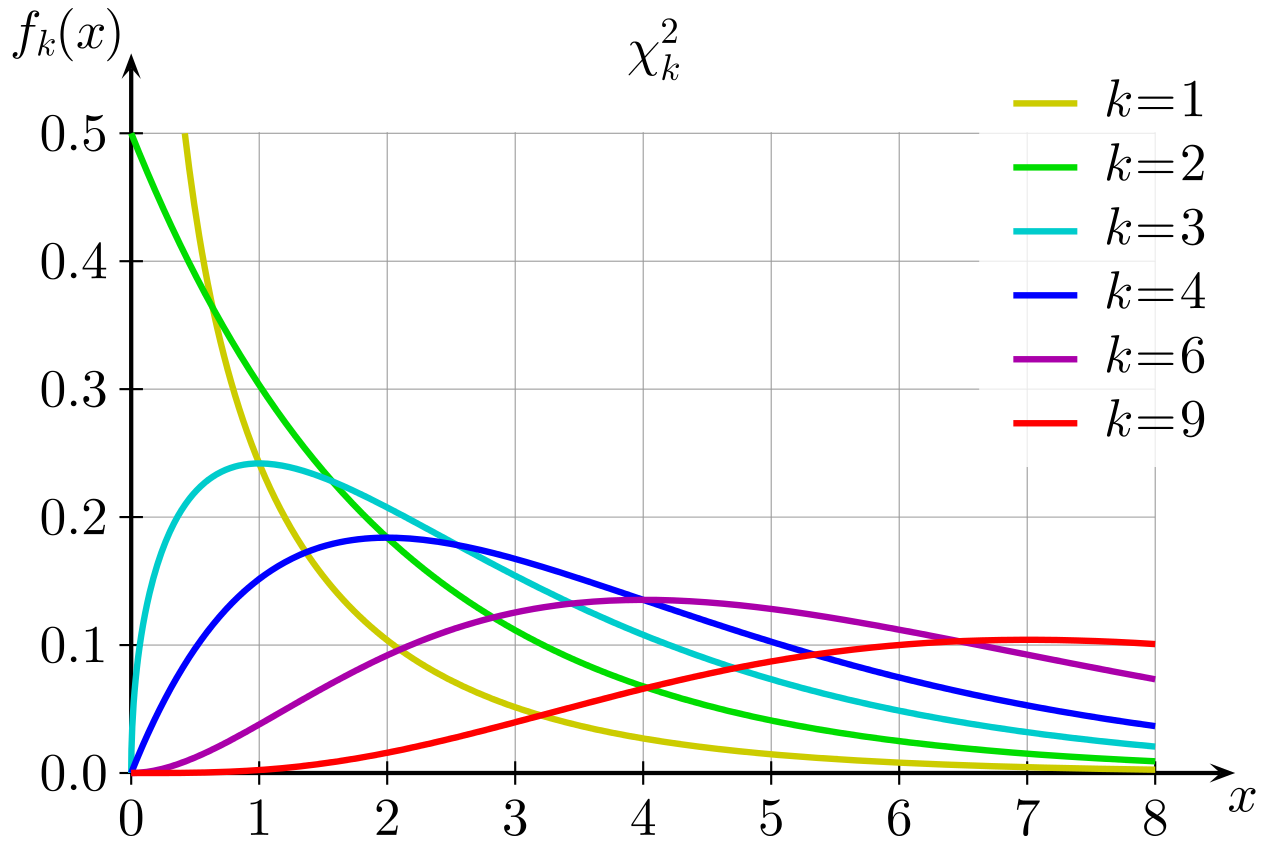
\includegraphics[height=0.38\textheight]{P05cpdf.png}
	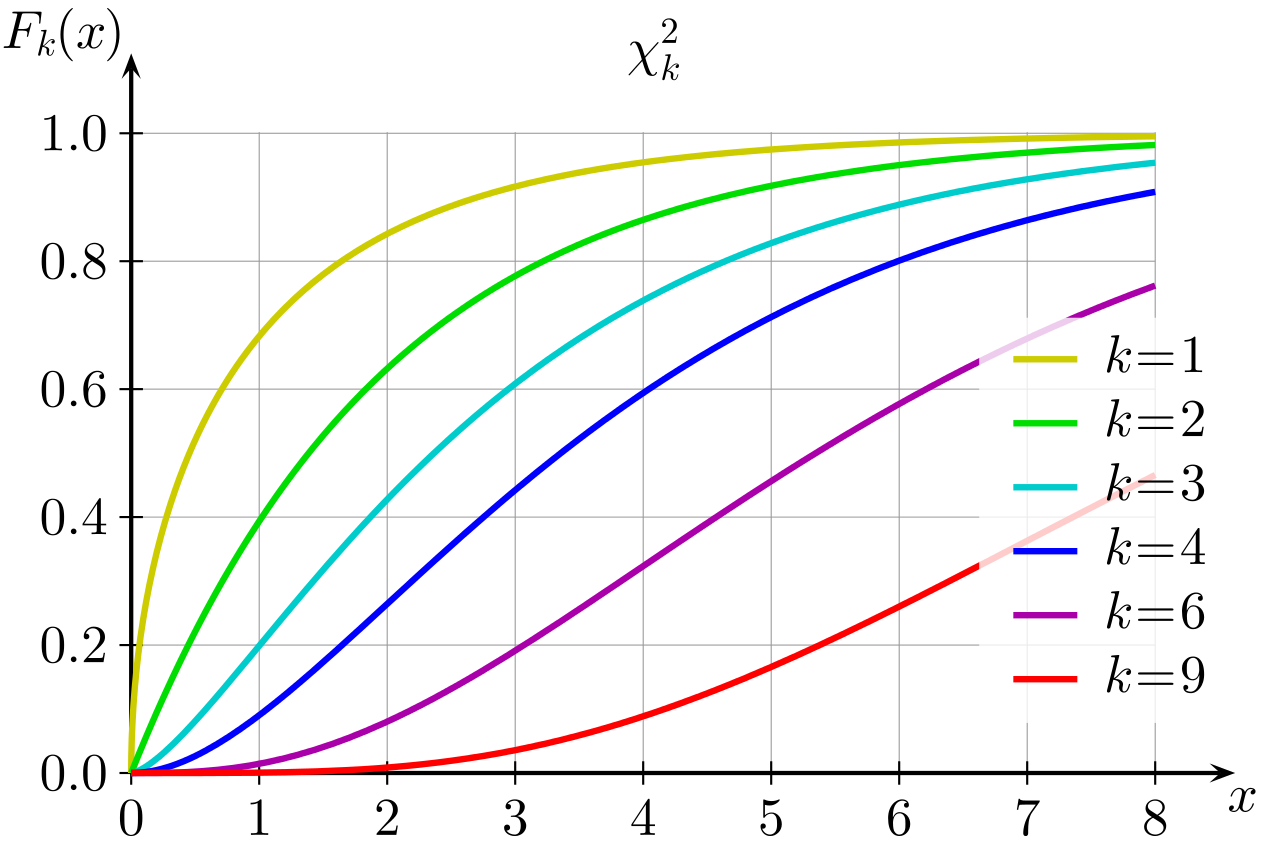
\includegraphics[height=0.38\textheight]{P06ccdf.png}}
	\credits{By Geek3 at Wikipedia Commons. CC BY 3.0.}
\end{exmp}
\pagebreak
%%%%%%%%%%%%%%%%%%%%%%%%%%%%%%%%
\begin{exmp}[F-distribution]{exmp:fdist}
	The Fisher–Snedecor or short F-distribution is the ratio of two, independent Chi-square distributions:
	\begin{equation*}
	X_1\sim \chi^2_{d_1},\;	X2_\sim \chi^2_{d_2}\;\rightarrow\;\frac{X_1/d_1}{X_2/d_2}\sim F(d_1,d_2)
	\end{equation*}
	
	\centering{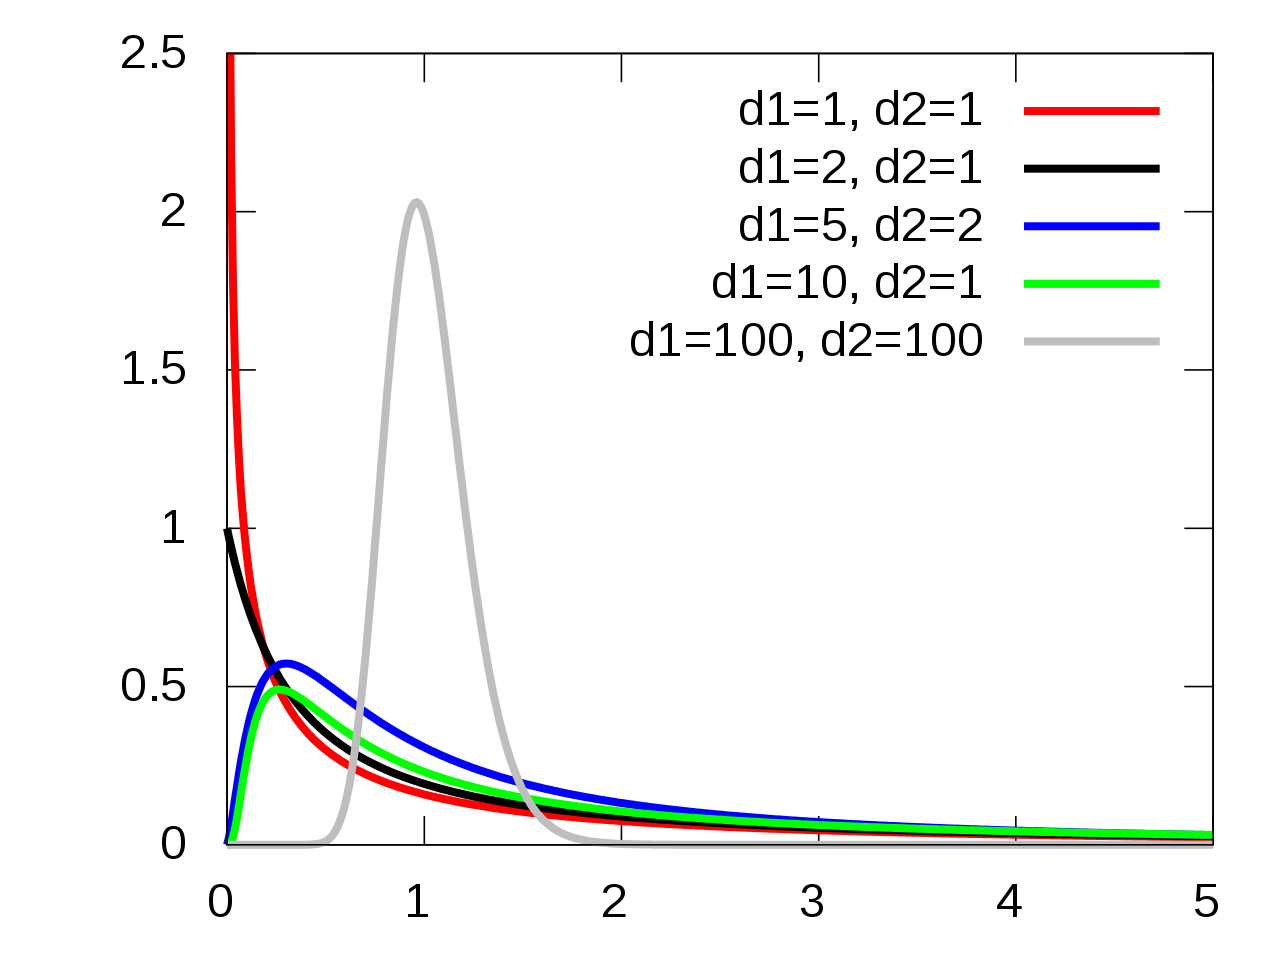
\includegraphics[height=0.35\textheight,width=0.8\textwidth]{P07fpdf.png}
	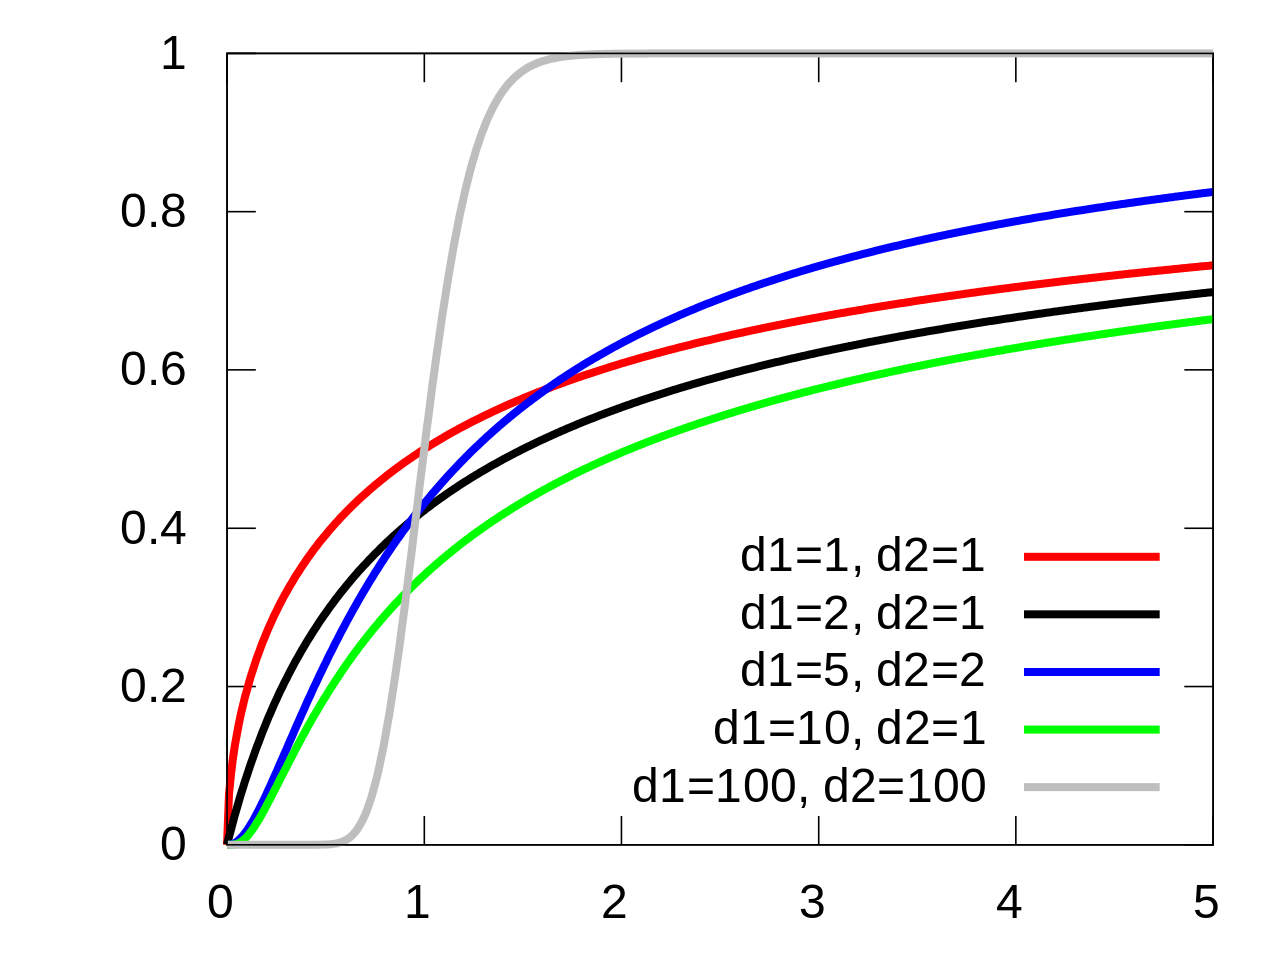
\includegraphics[height=0.35\textheight,width=0.8\textwidth]{P08fcdf.png}}		
	\credits{By IkamusumeFan at Wikipedia Commons. CC BY-SA 4.0.}
\end{exmp}